\documentclass[10pt,a4paper]{article}
\usepackage[utf8]{inputenc}
\usepackage[german]{babel}
\usepackage{mathrsfs}
\usepackage{amsmath}
\usepackage{amsfonts}
\usepackage{amssymb}
\usepackage{amsthm}
\usepackage[left=2cm,right=2cm,top=2cm,bottom=2cm]{geometry}
\usepackage{minted}
\usepackage{graphicx}

\begin{document}

\section{Aufgabe 6.1}

Damit sein Adressbereich nicht fragmentiert wird?

\section{Aufgabe 6.2}

Weil sich dadurch von außen die einzelnen Teilnehmer nicht unterscheiden lassen.

\section{Aufgabe 6.3}

Die Benutzer des Internetzugangs sehen von außen alle gleich aus. Dadurch kann
man nicht mehr herausfinden, wer etwaige Straftaten im Netz begangen hat. Um
dies zu umgehen, könnte man z.B. den Betreiber des Zugangs verpflichten, den
gesamten Verkehr mitzuschneiden und die Einstellungen des NAT und anderen
relevante Dinge (DHCP?) zu loggen.

\section{Aufgabe 6.4}

\subsection{Teil 1}

Historisch sind die erste und letzte Adresse eines Subnetzes
Broadcastadressen. Die erste kann jedoch frei verwendet werden, wenn keine
Windows-9x (95, 98, Me) im Netzwerk sind. Die zweite kann bei modernen
Betriebssystemen ebenfalls als Broadcastadresse deaktiviert werden, sodass alle
Adressen frei verfügbar sind. (Quelle: wikipedia:Subnetz)

\subsection{Teil 2}

Ein Subnetz mit Subnetzmaske $x$ hat $32 - x$ frei wählbare Bits. Es sind also
$2^{32 - x}$ im Subnetz verfügbar.

\subsection{Teil 3}

Insgesamt haben wir $2^{7} = 128$ Adressen. Das kann man aufteilen in 4 Subnetze
mit $64$, $32$ und zwei mal $16$ Adressen.

\begin{figure}[h]
  \centering
  \begin{tabular}{lrrrr}
    & 64 & 32 & 16 & 16\\
    \hline
    netid & 91.192.100.128 & 91.192.100.192 & 91.192.100.224 & 91.192.100.240\\
    netmask & 255.255.255.192 & 255.255.255.224 & 255.255.255.240 & 255.255.255.240\\
    CIDR suffix & 26 & 27 & 28 & 28\\
    broadcast & 91.192.100.191 & 91.192.100.223 & 91.192.100.239 & 91.192.100.255\\
    max num add & 63 & 31 & 15 & 15\\
  \end{tabular}
\end{figure}

\section{Aufgabe 6.5}

\begin{minted}{c}
  int maskBytes; // 24 bei 1.1.1.1/24
  int addr1;
  int addr2;
  int mask = (-1) << (32 - maskBytes); // Subnetzmaske

  (addr1 & mask) - (addr2 & mask) == 0;
\end{minted}

\section{Aufgabe 6.6}

\subsection{Teil 1}

Weil man von außen durch ein NAT nicht ohne weiteres eine Verbindung aufbauen
kann.

\subsection{Teil 2}

Cindy könnte quasi zwischen den beiden vermitteln, indem sie Bernhard mitteilt,
dass er sich bei Arnold melden soll.

\subsection{Teil 3}

Die Lösung von gerade funktioniert nun nicht mehr, weil auch Arnold hinter einem
NAT sitzt.

\section{Aufgabe 6.7}

\subsection{Teil 1}

Jede WG kriegt einen Router mit DHCP und wir machen Distance-Vector-Routing, um
die sich oft ändernden Verhältnisse gut abfangen zu können.

\subsection{Teil 2}

\begin{figure}[h]
  \centering
  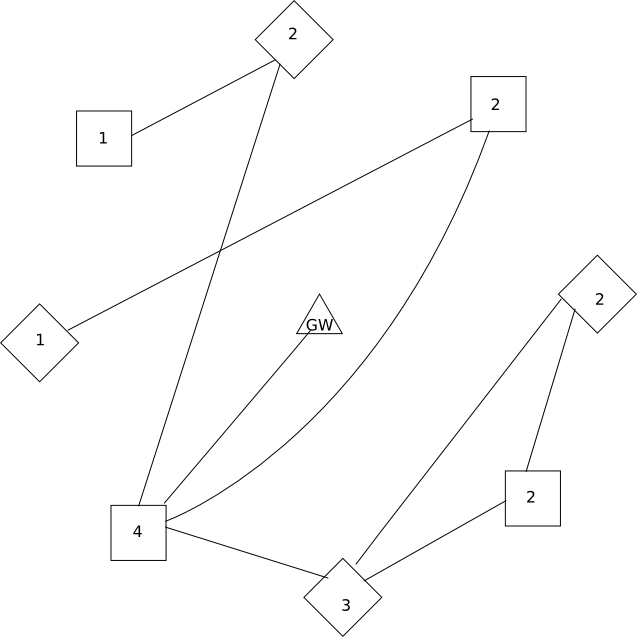
\includegraphics[width=350pt]{6_7_b}
\end{figure}
Bei dieser Konfiguration kann jeder jeden erreichen. Dabei gibt es aber nur in
dem Dreieck unten rechts Redundanz.

\section{Aufgabe 6.8}

\begin{figure}[h]
  \centering
  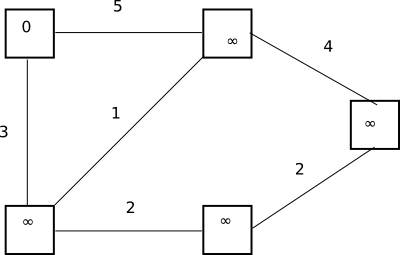
\includegraphics[width=200pt]{6_8_1}
  \caption{Initialzustand}
\end{figure}
\begin{figure}[h]
  \centering
  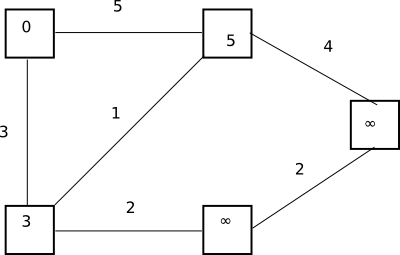
\includegraphics[width=200pt]{6_8_2}
  \caption{Update 1}
\end{figure}
\begin{figure}[h]
  \centering
  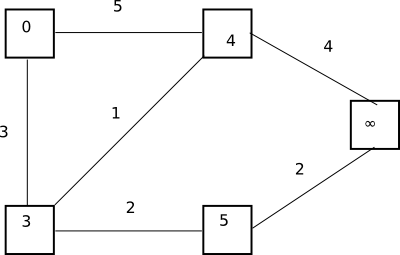
\includegraphics[width=200pt]{6_8_3}
  \caption{Update 2}
\end{figure}
\begin{figure}[h]
  \centering
  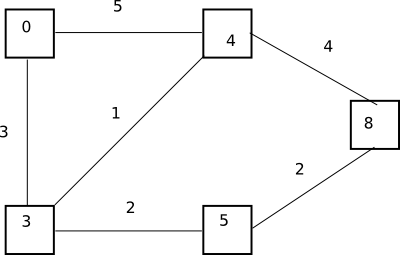
\includegraphics[width=200pt]{6_8_4}
  \caption{Update 3}
\end{figure}
\begin{figure}[h]
  \centering
  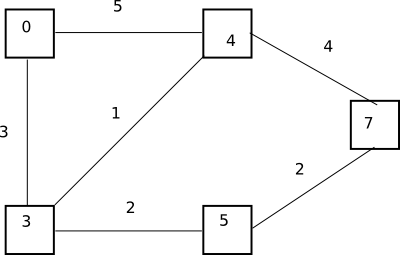
\includegraphics[width=200pt]{6_8_5}
  \caption{Update 4 und Endzustand}
\end{figure}

\end{document}